\documentclass[12pt]{article}
	\usepackage{amsmath}
	\usepackage{amssymb}
	\usepackage{fancyhdr}
	\usepackage{float}
	\usepackage{graphicx}
	\usepackage{cite}

	\oddsidemargin0cm
	\topmargin-2cm     %I recommend adding these three lines to increase the 
	\textwidth16.5cm   %amount of usable space on the page (and save trees)
	\textheight23.5cm  

\newcommand{\myname}{Evan Palmer, Titouan Rigoudy}
\newcommand{\myandrew}{esp@andrew, trigoudy@andrew}
\newcommand{\myhwnum}{1}
\newcommand{\problemnum}{1}
\newcommand{\thedate}{\today}
\DeclareMathOperator*{\argmax}{arg\,max}
%Page header
	\setlength{\parindent}{0pt}
	\setlength{\parskip}{5pt plus 1pt}
	 
	\pagestyle{fancyplain}
	\lhead{\fancyplain{}{\textbf{Project midway report}}}      % Note the different brackets!
	\rhead{\fancyplain{}{\myname\\ \myandrew}}
	\chead{\fancyplain{}{10-701}}
\begin{document}
%Title
	\medskip    
	\thispagestyle{plain}
	\begin{center}                 
	{\LARGE Finding The Best Critic For You} \\
	\medskip
	Machine Learning Midway Report \\
	\smallskip
	\myname \\
	\myandrew \\
	\thedate \\
	\end{center}
	\vspace{0.5cm}

\section{Introduction}

\section{Obtaining the data}

	We found two sites public API where we could access movie information and reviews: Rotten Tomatoes and Metacritic. We wanted to find movies which many critics and users would likely have seen and rated. Unfortunately neither of these sites had a mechanism for retrieving the most reviewed films. 

	To solve this problem we obtained a list of the most rated films from IMDb. We sorted this list by the number of ratings, and chose the five thousand most rated movies. 

	We then used the Metacritic and Rotten Tomatoes APIs to retrieve information, reviews, and anything else that was available for each of these movies.

\section{Data descriptions}

\subsection{Rotten Tomatoes}

	The data we retrieved from Rotten Tomatoes included 520068 reviews of 4538 movies by 4474 critics. Of all these reviews, 101492 were identified as ``top'' reviews. These were written by 1343 different critics.

	The Rotten Tomatoes data is very promising. Movies are reviewed by on average about twenty critics which are designated as \textit{top critics}, and by about one hundred critics with no top designation. Furthermore, these distributions are fairly uniform as shown by the Histogram in Figure \ref{fig:r_mov}. This means that we have a large number of movies with many critic reviews.

	Critics have, on average about twenty reviews where they are designated as \textit{top critics}, and about seventy where they receive no designation. This might seem surprising as we would expect top critics to review more things. Really this reflects an interesting naming convention by Rotten Tomatoes. Though a critic may be designated as a \textit{top critic} for a particular movie, this designation may change from movie to movie. One notable exception is Rodger Ebert who was designated as a top critic for $2862$ movies! These distributions are more skewed by critics, like Ebert, who have reviewed many movies as seen in Figure \ref{fig:r_crit}. However, there are still many critics who have reviewed a sizable number of films.

	Rotten Tomatoes differentiates between individual critics and the publication which they write for. If we look at the same things we looked at for critics, but group them by publication, we find a higher mean number of films reviewed. This could be useful as publications, like critics, may maintain a distinct taste profile.

	\begin{table}[H]
	 \centering
	 \caption{Distribution of number of reviews per critic for movies on rotten tomatoes}
	 \begin{tabular}{ l | c | c | c | c }
	 \hline
	 &  Min & Max & Mean & Std Dev  \\
	 \hline
	 Top Critcs & 0 & 56 & 22.41 & 16.06 \\
	 Other Critics & 0 & 316 & 92.24 & 68.12 \\
	 \hline
	 \end{tabular}
	 \end{table}

	\begin{figure}[H]
	    \centering
	    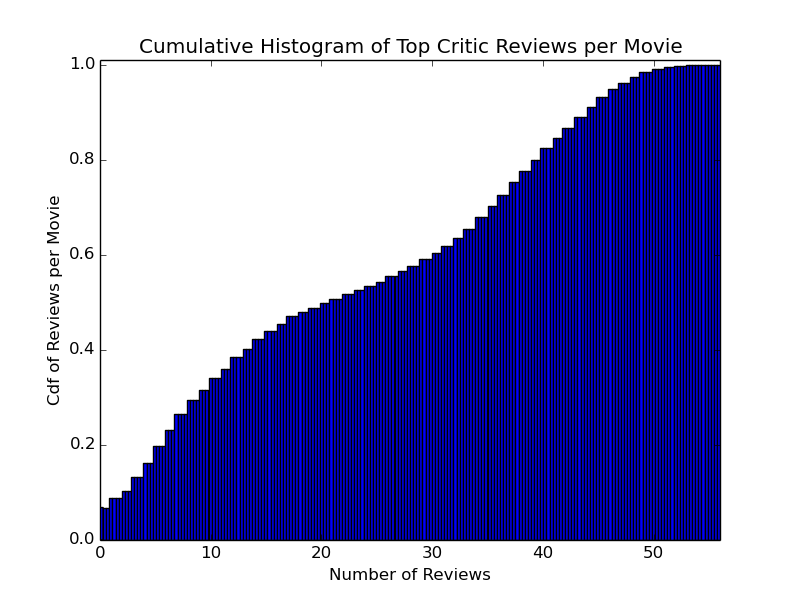
\includegraphics[width=0.48\textwidth]{plots/plot_r_mov_top.png}
	    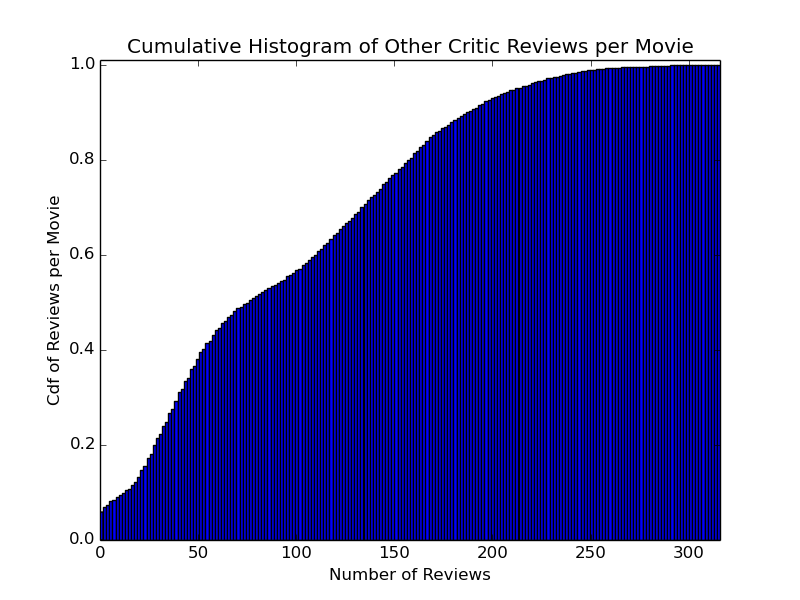
\includegraphics[width=0.48\textwidth]{plots/plot_r_mov_oth.png}
	    \caption{Cumulative histograms of critic reviews per movie for movies on Rotten Tomatoes}
	    \label{fig:r_mov} 
	\end{figure}


	\begin{table}[H]
	 \centering
	 \caption{Distribution of number of reviewed movies per critic on rotten tomatoes} 
	 \begin{tabular}{ l | c | c | c | c }
	 \hline
	 &  Min & Max & Mean & Std Dev  \\
	 \hline
	 Top Critcs & 0 & 2862 & 21.79 & 124.96 \\
	 Other Critics & 0 & 2634 & 68.16 & 224.77 \\
	 \hline
	 \end{tabular}
	 \end{table}

	\begin{figure}[H]
	    \centering
	    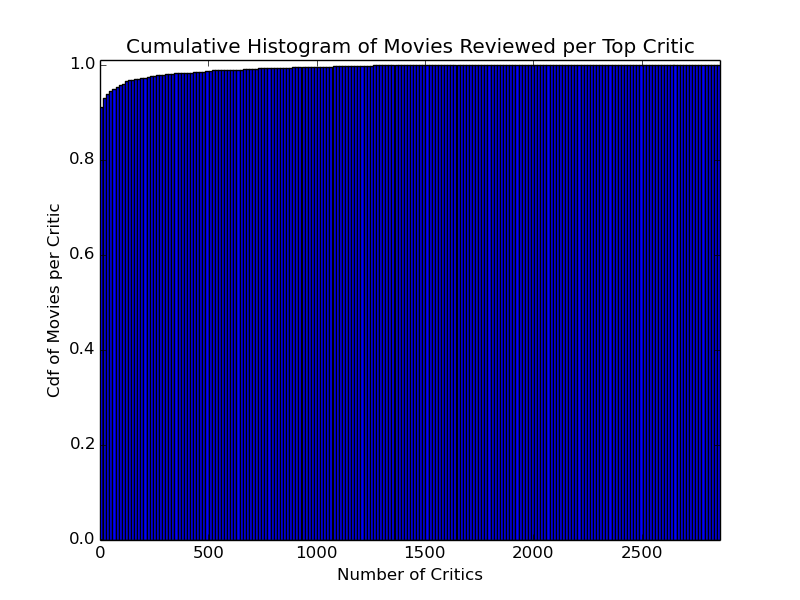
\includegraphics[width=0.48\textwidth]{plots/plot_r_crit_top.png}
	    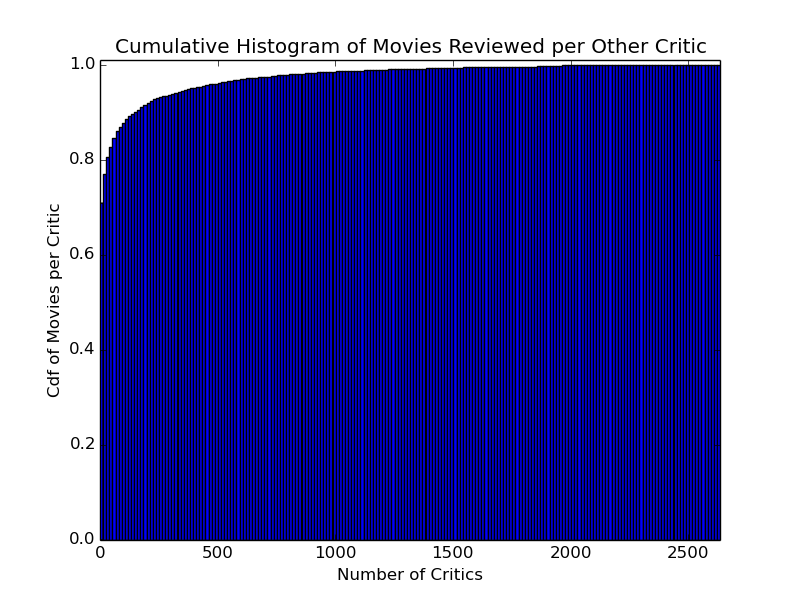
\includegraphics[width=0.48\textwidth]{plots/plot_r_crit_oth.png}
	    \caption{Cumulative histograms of the number of movies reviewed by critics on Rotten Tomatoes}
	    \label{fig:r_crit}
	\end{figure}


	\begin{table}[H]
	 \centering
	 \caption{Distribution of number of reviewed movies per publication on rotten tomatoes} 
	 \begin{tabular}{ l | c | c | c | c }
	 \hline
	 &  Min & Max & Mean & Std Dev  \\
	 \hline
	 Top Publications & 0 & 4135 & 97.22 & 454.15 \\
	 Other Publications & 0 & 3224 & 297.78 & 520.28 \\
	 \hline
	 \end{tabular}
	 \end{table}

	 \begin{figure}[H]
	    \centering
	    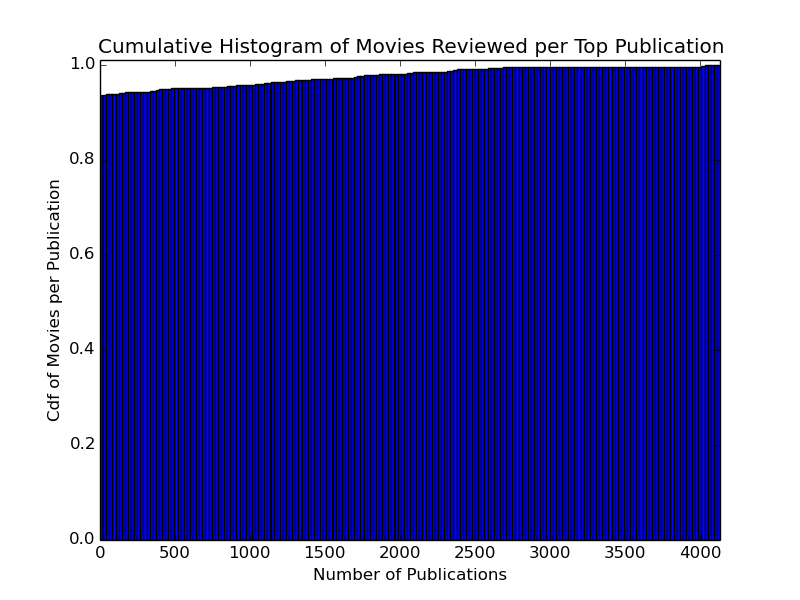
\includegraphics[width=0.48\textwidth]{plots/plot_r_pub_top.png}
	    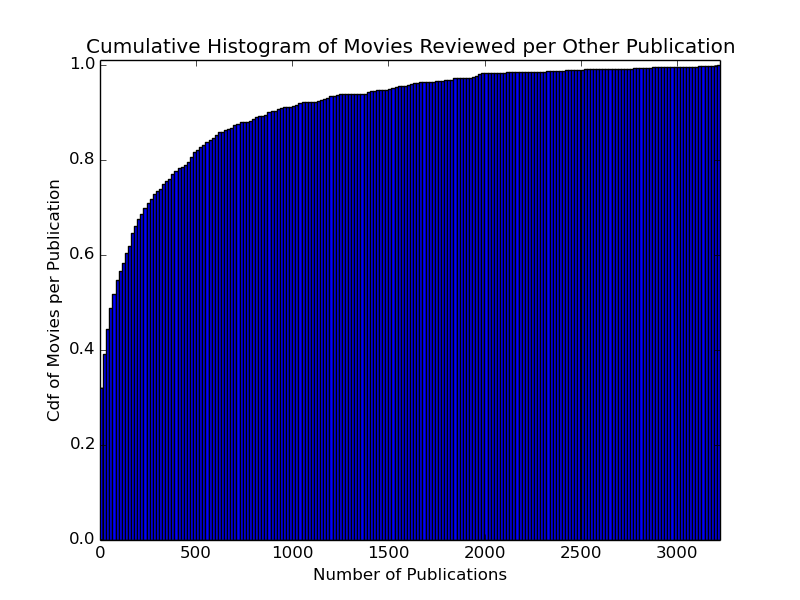
\includegraphics[width=0.48\textwidth]{plots/plot_r_pub_oth.png}
	    \caption{Cumulative histograms of the number of movies reviewed by publications on Rotten Tomatoes}
	    \label{fig:r_pub}
	\end{figure}

\subsection{Metacritic}

	The Metacritic dataset contains $3228$ movies with $152622$ reviews from $69$ unique critics and $20183$ unique users. Of these reviews $80332$ were written by users, and $69590$ were written by critics


	Films were somewhat harder to retrieve from Metacritic than Rotten Tomatoes. The indexing in the Metacritic search function seemed to rely mostly on attributes other than title, as a result, many queries resulted in the wrong movie. For instance when searching for \textit{Batman Begins} we instead received \textit{The Dark Knight}. This is most likely due to \textit{Batman} being very closely related to \textit{The Dark Knight}, and the film \textit{Batman Begins} being significantly less popular. Due to problems like this we were unable to retrieve as many films as with Rotten Tomatoes.

	In contrast to rotten tomatoes, Metacritic draws from a very small pool of critics. This is partially because what Metacritic describes as \textit{critics} Rotten Tomatoes describes as \textit{publications}. On average each of these critics has reviewed twelve hundred films. This means that for each critic we have a fairly large overlap.

	The films also have about twenty one user reviews on average. This provides us with real user data which is something which we did not obtain from Rotten Tomatoes. As seen in Figure \ref{fig:m_crit}, Approximately twenty percent of movies have at least twenty user reviews, giving us a reasonable number of movies with reviews.

	Unfortunately, there are very few users who review many movies. From Figure \ref{fig:m_crit} we can see that reviewing more than twenty films occurs at approximately the ninety-eighth percentile, giving us about forty users.

	\begin{table}[H]
	 \centering
	 \caption{Distribution of number of reviews by users and critics for movies on Metacritic}

	 \begin{tabular}{ l | c | c | c | c }
	 \hline 
	 &  Min & Max & Mean & Std Dev  \\
	 \hline
	 Critics with reviews & 0 & 49 & 25.72 & 10.83 \\
	 Users with reviews & 0 & 842 & 21.56 & 50.05 \\
	 \hline
	 \end{tabular}
	 \end{table}

	 \begin{figure}[H]
	    \centering
	    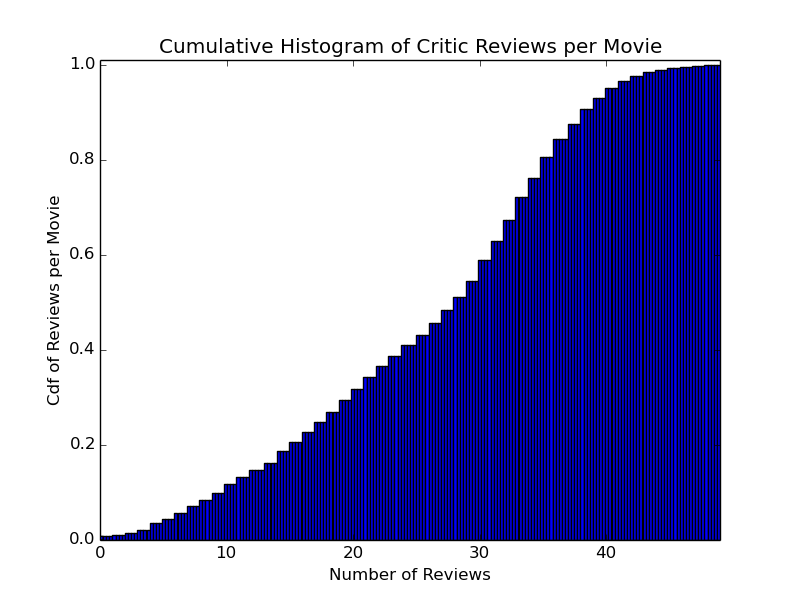
\includegraphics[width=0.48\textwidth]{plots/plot_m_mov_top.png}
	    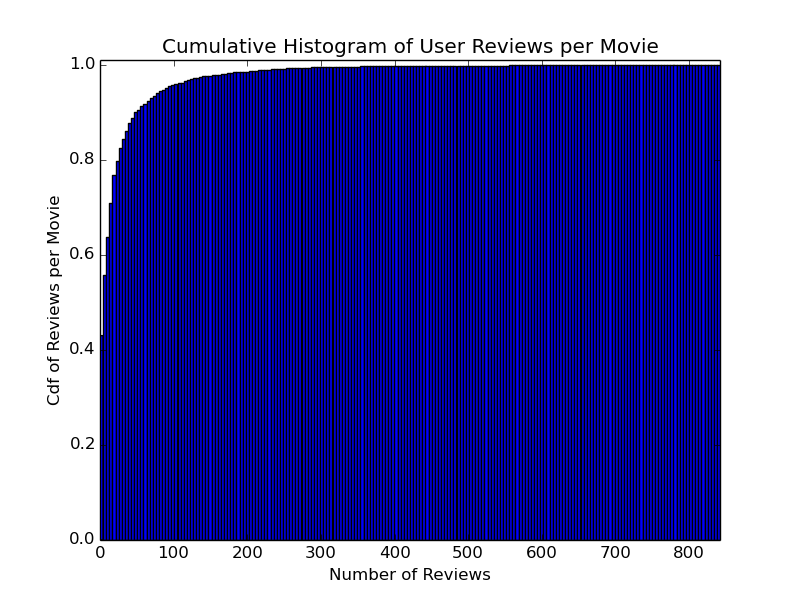
\includegraphics[width=0.48\textwidth]{plots/plot_m_mov_usr.png}
	    \caption{Cumulative histograms of critic and user reviews per movie for movies on Metacritic}
	    \label{fig:m_mov}
	\end{figure}


	\begin{table}[H]
	\centering
	 \caption{Distribution of number of reviewed movies by users and critics on Metacritic}

	 \begin{tabular}{ l | c | c | c | c }
	 \hline
	 &  Min & Max & Mean & Std Dev  \\
	 \hline
	 Reviews per critic & 56 & 3445 & 1203.36 & 912.50 \\
	 Reviews per user & 1 & 536 & 3.45 & 14.55 \\
	 \hline
	 \end{tabular}
	 \end{table}


	 \begin{figure}[H]
	    \centering
	    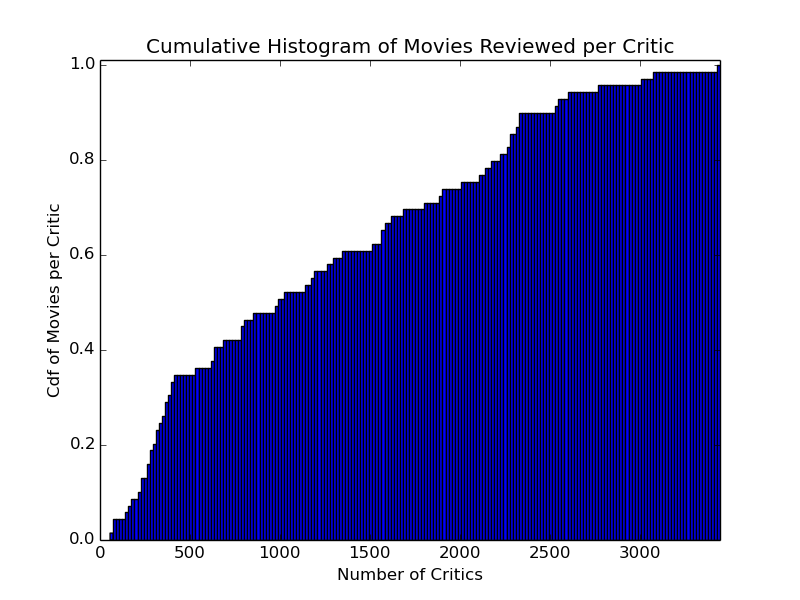
\includegraphics[width=0.48\textwidth]{plots/plot_m_crit_top.png}
	    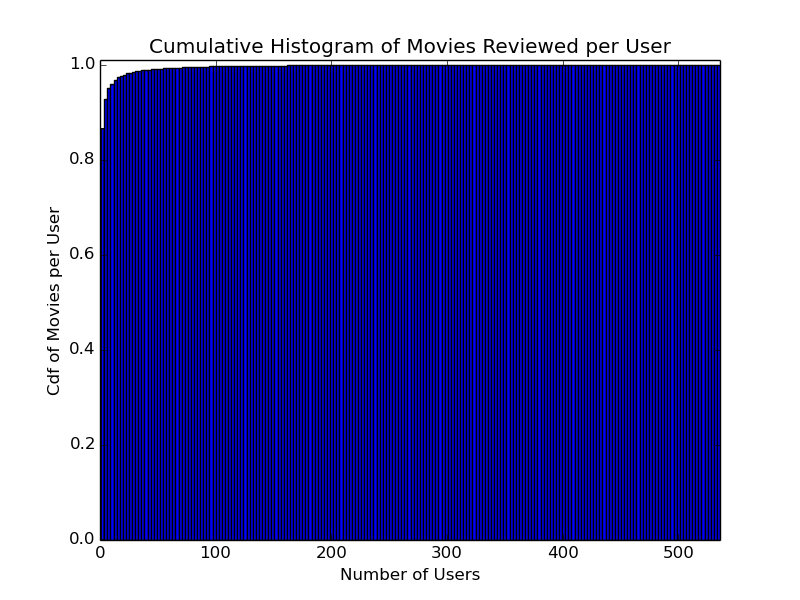
\includegraphics[width=0.48\textwidth]{plots/plot_m_crit_usr.png}
	    \caption{Cumulative histograms of the number of movies reviewed by users and critics on Metacritic}
	    \label{fig:m_crit}
	\end{figure}

\section{Recommender Systems}

What we are trying to do for this project is to recommend a critic to a user based on past critic ratings and past user ratings. In other words, we are trying to build a recommender system.

Formally, a recommender system takes a set of users $U = \{u_1, ..., u_N\}$, a
set of items $I = \{i_1, ..., i_M\}$, and a sparse matrix of ratings
$R$ of size $N \times M$. If $R_{k,l} > 0$, then user $u_k$ has given item $i_l$ a rating of $R_{k,l}$. A zero rating signifies that the
user has not rated the item. The goal of the system is then to predict the rating that a user would give to an item he has not yet rated. The system can
then recommend any number of items with highest predicted rating.

As described in \cite{Survey05}, recommender systems can be divided in three broad categories: content-based systems, collaborative systems and hybrid systems. 

Content-based recommender systems try to identify item features in order to compare items and recommend similar items to those that the user has rated highly in the past.  For example, if a user consistently rates history books highly, the system can recommend other history books.

Collaborative recommender systems do not try to extract features from the items
to be recommended. Instead, such systems will recommend items that users with similar tastes have rated highly in the past.

Hybrid recommender systems try to combine both approaches in order to improve recommendations.

Our particular problem places a twist on the conventional recommendation problem, as we are not trying to recommend movies to users, but rather recommend critics to users. Movie ratings serve as an indirect measure of similarity that we want to use in order to provide good recommendations. Still, the main problem of overcoming rating sparsity remains a focal point.

\section{Matrix factorization}

Our first approach was to try to learn movie features and critic features, as if we were training a content-based movie recommendation system. The idea was that using the learned critic features, we could then hope to easily compare critics by simply comparing their feature vectors, which would completely describe their tastes. By then learning user features with the same movie features, we could then hope to compare users' and critics' tastes, and therefore recommend critics to users. 

We decided to learn critic and movie features through matrix factorizaton, as described by Koren, Bell and Volinsky in \cite{Koren09}. Their paper describes an a content-based recommender system which learns user and item features by modeling the ratings matrix as the product of an user feature matrix and an item feature matrix. This translates to the following minimization problem:
$$ \min_{U,I} \sum_{k = 1}^{N} \sum_{l = 1}^{M} (R_{k,l} - U_k I_l^T)^2 + \lambda (||U||_2^2 + ||I||_2^2) $$
Where $U$ is a $N \times D$ matrix of user features, $U_k$ is the k-th row of $U$, $I$ is a $M \times D$ matrix of item features, $I_l$ is the l-th row of $I$, and $D$ is a tunable number of dimensions.

Calculating the gradient of this sum of $NM$ terms in turn requires the calculation of the sum of $NM$ terms. In our case, for the Rotten Tomatoes data, $N = 4474$ and $M = 4538$, which means that we would need to sum over 20 million terms for each gradient calculation. Running batch gradient descent on that data would therefore be too slow for our needs, considering the computational power at our disposal. As also described in \cite{Koren09}, we therefore decided to use stochastic gradient descent as our minimization algorithm, which only calculates the gradient of one term of the huge sum at each iteration.


	\begin{figure}[H]
	\centering
	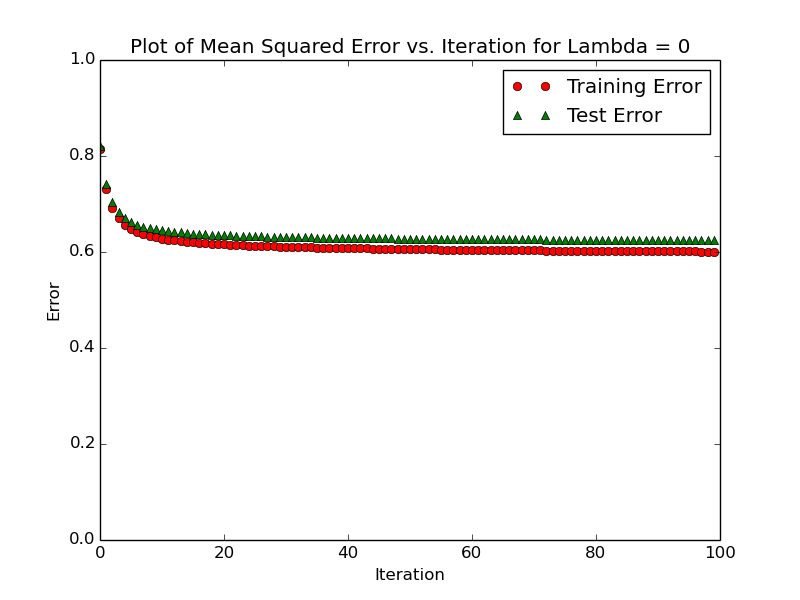
\includegraphics[width=0.48\textwidth]{plots/test-i100d1l0.png}
	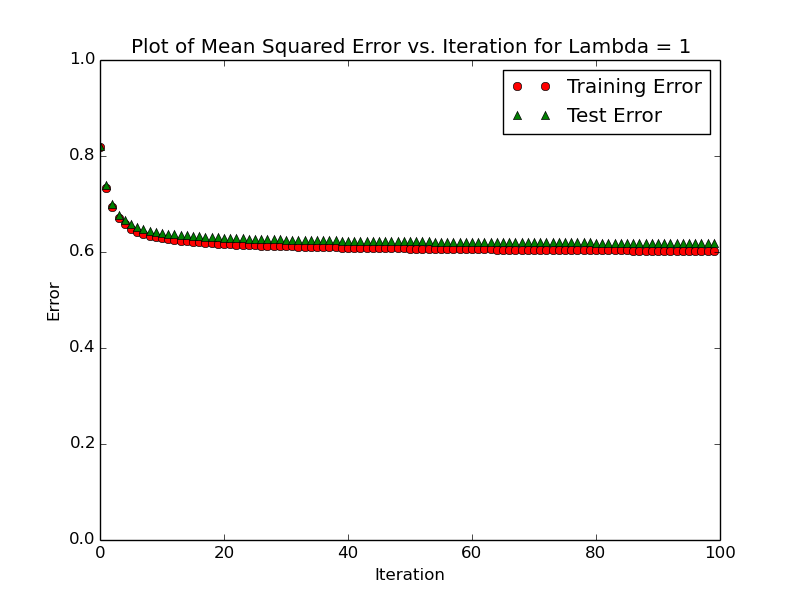
\includegraphics[width=0.48\textwidth]{plots/test-i100d1l1.png}
	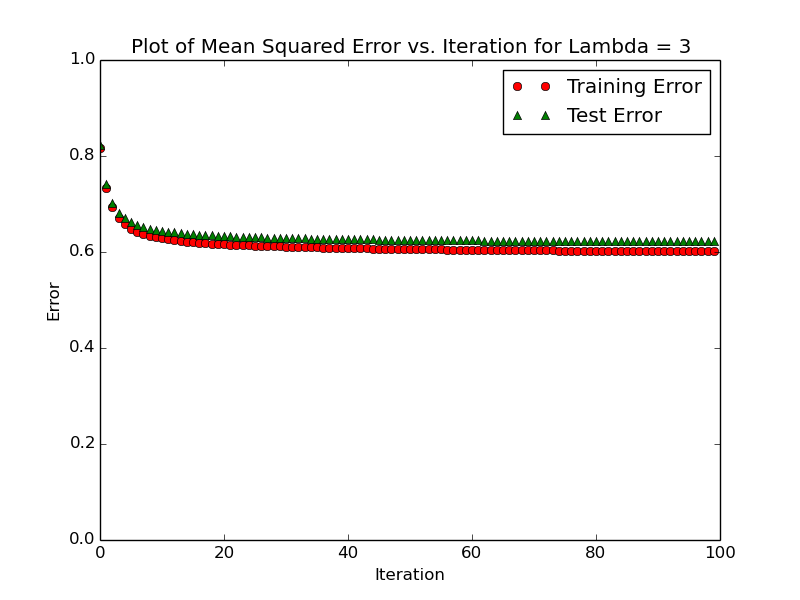
\includegraphics[width=0.48\textwidth]{plots/test-i100d1l3.png}
	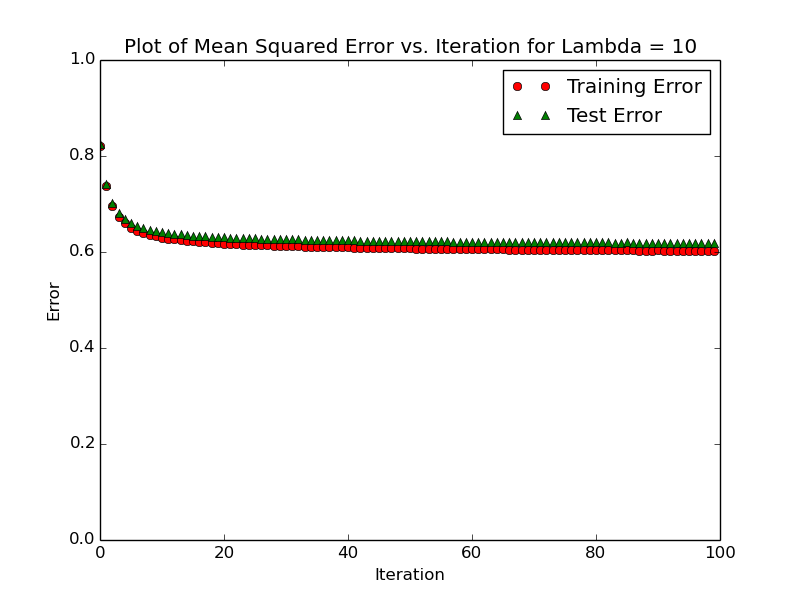
\includegraphics[width=0.48\textwidth]{plots/test-i100d1l10.png}
	\caption{Mean squared training and test error over 100 iterations in the stochastic matrix factorization model. Stochastic gradient descent was done using a step size of 0.02. The learned critic matrix was count(critics) by 1, and the learned movie matrix was 1 by count(movies).}
	\label{fig:1}
	\end{figure}


	\begin{figure}[H]
	\centering
	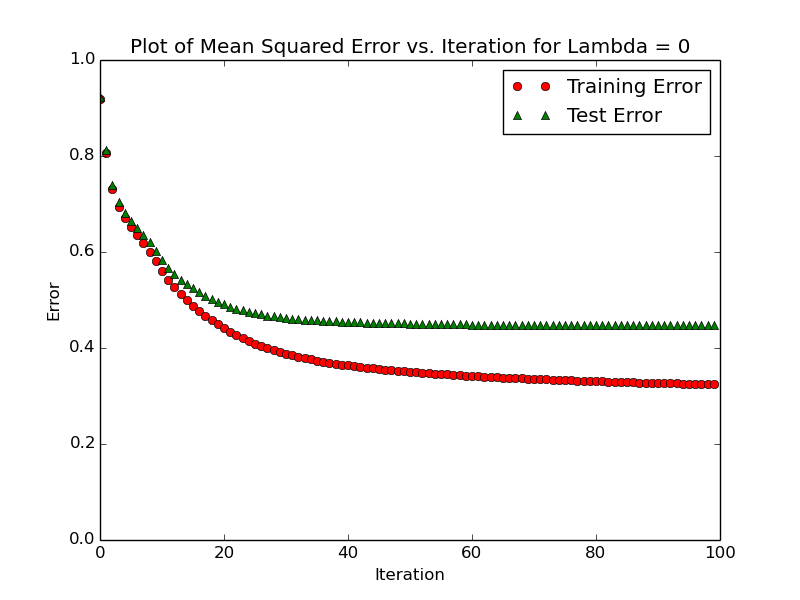
\includegraphics[width=0.48\textwidth]{plots/test-i100d10l0.png}
	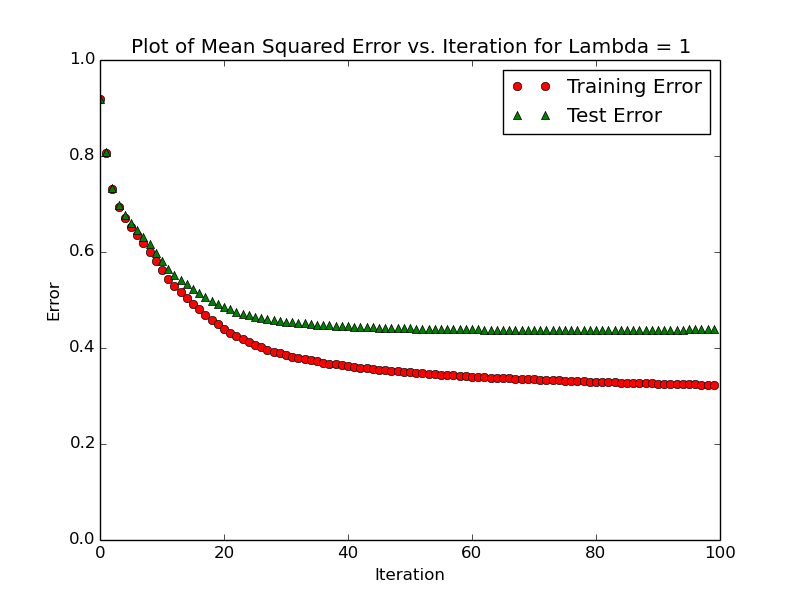
\includegraphics[width=0.48\textwidth]{plots/test-i100d10l1.png}
	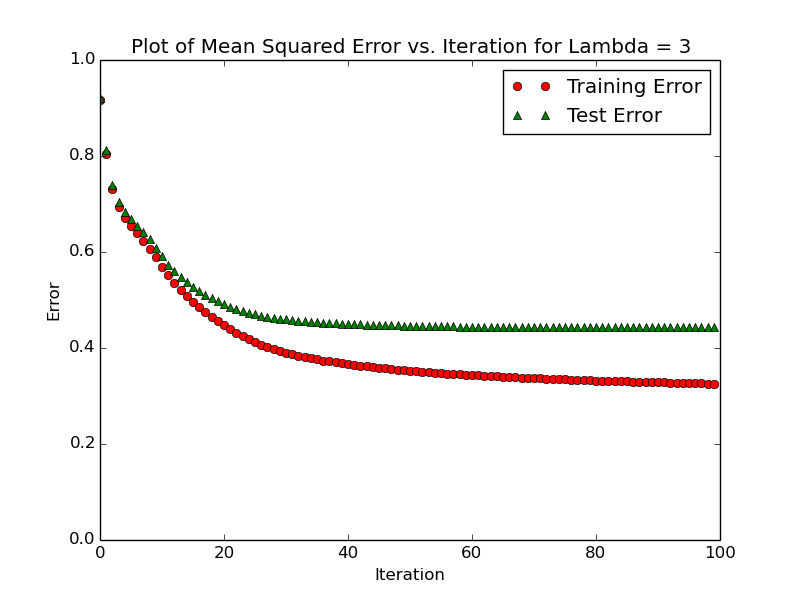
\includegraphics[width=0.48\textwidth]{plots/test-i100d10l3.png}
	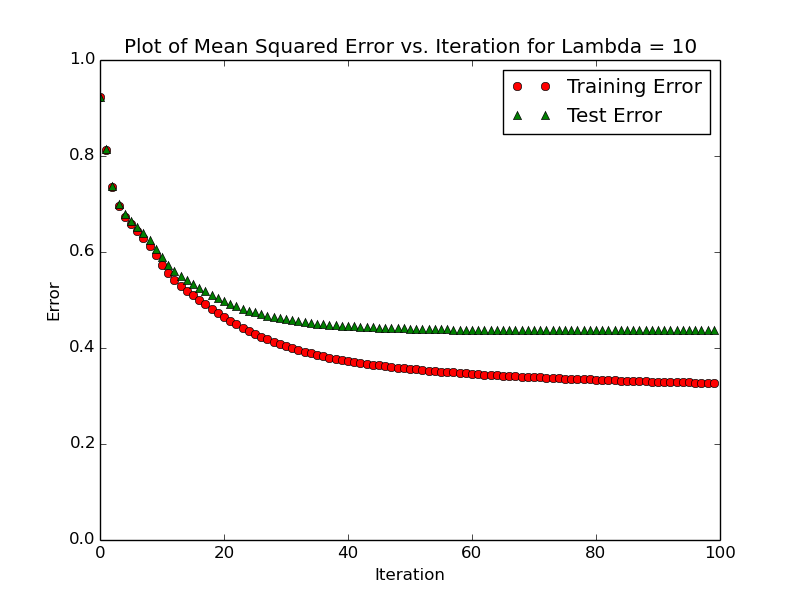
\includegraphics[width=0.48\textwidth]{plots/test-i100d10l10.png}
	\caption{Mean squared training and test error over 100 iterations in the stochastic matrix factorization model. Stochastic gradient descent was done using a step size of 0.02. The learned critic matrix was count(critics) by 10, and the learned movie matrix was 10 by count(movies).}
	\label{fig:10}
	\end{figure}


	\begin{figure}[H]
	\centering
	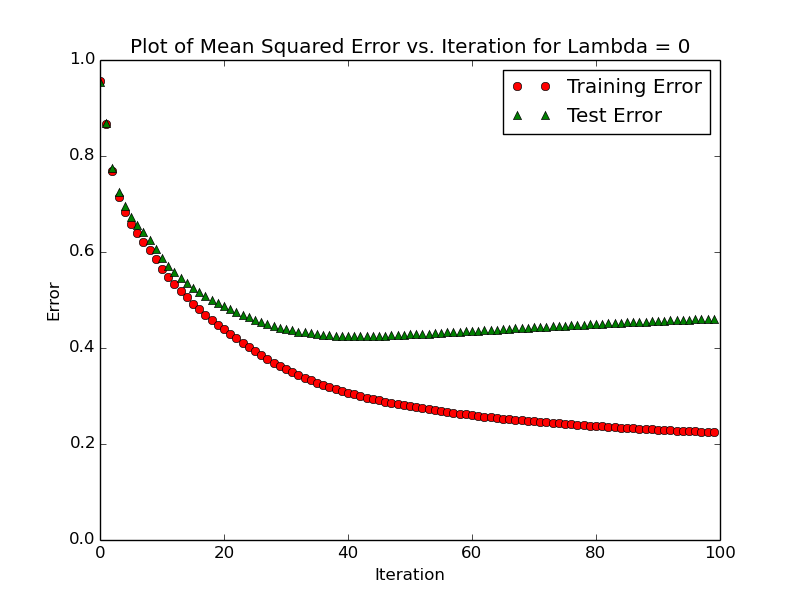
\includegraphics[width=0.48\textwidth]{plots/test-i100d25l0.png}
	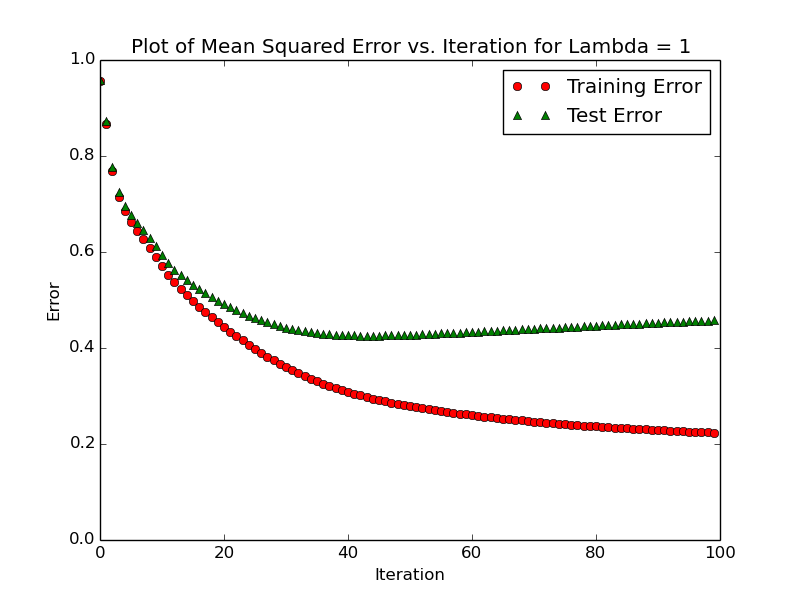
\includegraphics[width=0.48\textwidth]{plots/test-i100d25l1.png}
	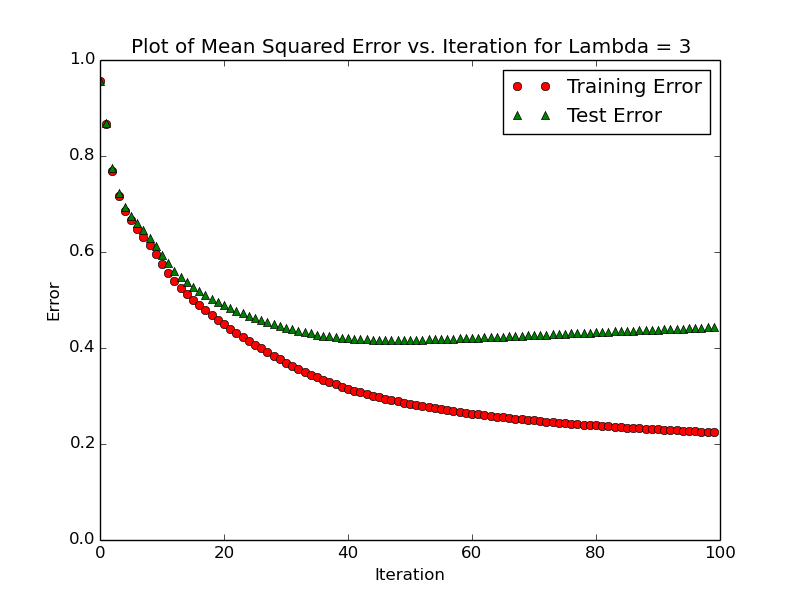
\includegraphics[width=0.48\textwidth]{plots/test-i100d25l3.png}
	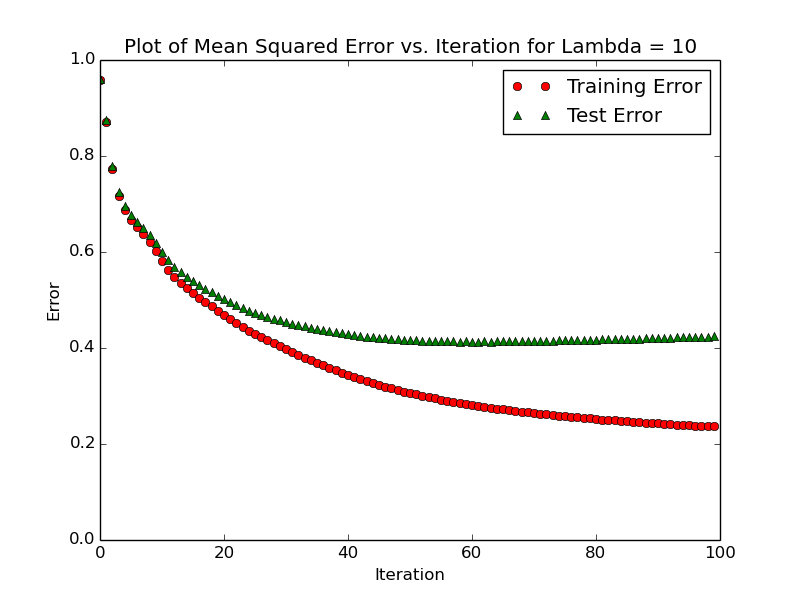
\includegraphics[width=0.48\textwidth]{plots/test-i100d25l10.png}
	\caption{Mean squared training and test error over 100 iterations in the stochastic matrix factorization model. Stochastic gradient descent was done using a step size of 0.02. The learned critic matrix was count(critics) by 25, and the learned movie matrix was 25 by count(movies).}
	\label{fig:25}
	\end{figure}


	\begin{figure}[H]
	\centering
	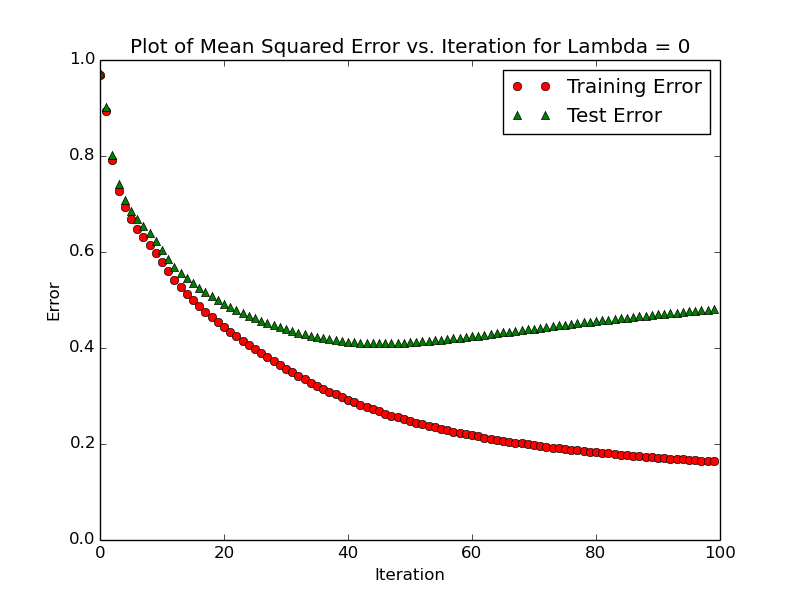
\includegraphics[width=0.48\textwidth]{plots/test-i100d40l0.png}
	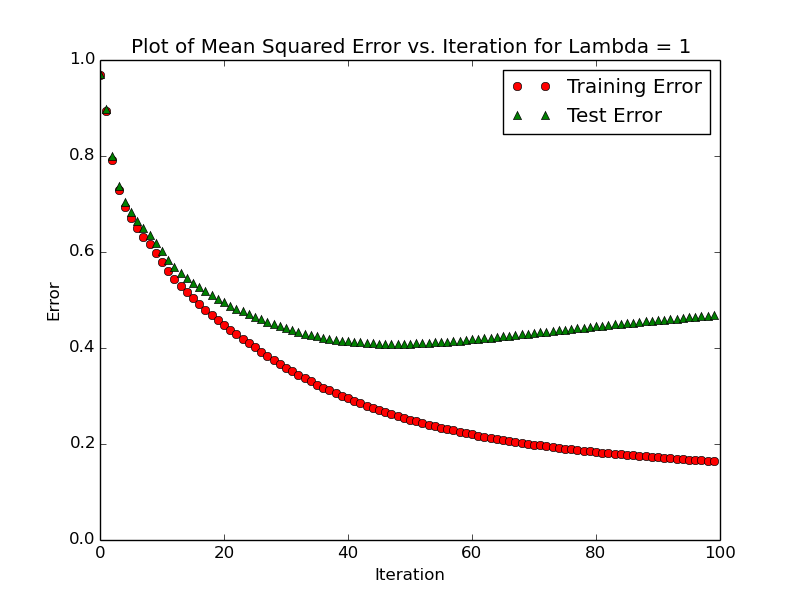
\includegraphics[width=0.48\textwidth]{plots/test-i100d40l1.png}
	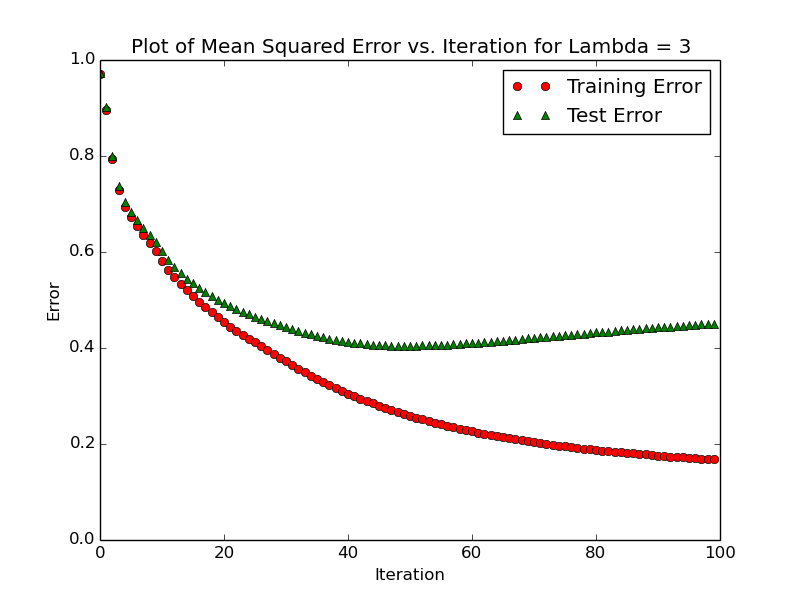
\includegraphics[width=0.48\textwidth]{plots/test-i100d40l3.png}
	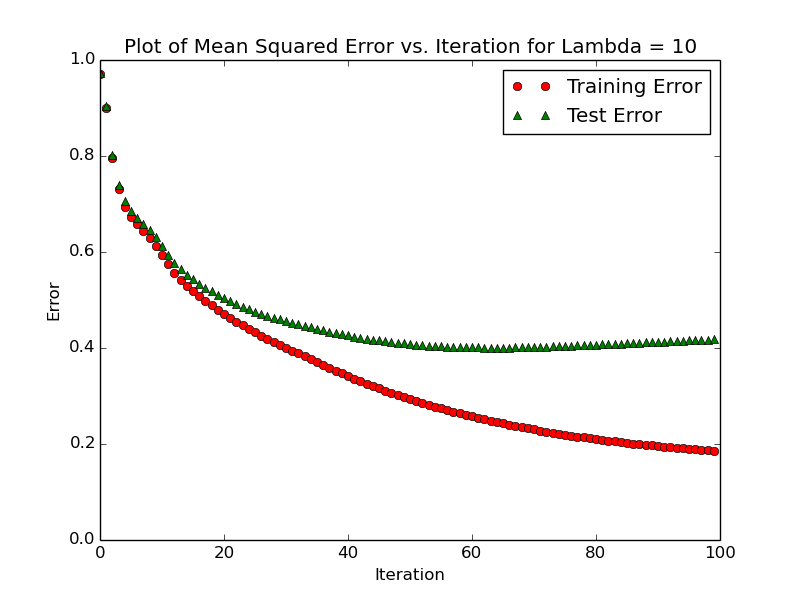
\includegraphics[width=0.48\textwidth]{plots/test-i100d40l10.png}
	\caption{Mean squared training and test error over 100 iterations in the stochastic matrix factorization model. Stochastic gradient descent was done using a step size of 0.02. The learned critic matrix was count(critics) by 40, and the learned movie matrix was 40 by count(movies).}
	\label{fig:40}
	\end{figure}


\section{Further work}

There are currently three big axes in which we want to extend our work.

The first axis is to extend our pure content-based system with collaborative elements, thus building a hybrid system. We have started work in that direction, by directly calculating a measure of similarity between critics based on ratings. The current implementation uses a cosine similarity measure between critic rating vectors, but it was not ready for this report. We plan on trying a correlation-based similarity measure and an adjusted cosine similarity measure, as described by Sarwar et al. in \cite{Sarwar01}.

The second extension would be to extract more features from data we already have (review publication, movie director, cast, runtime, MPAA rating, etc.) and integrate them in our matrix factorization model. Adding these fixed features to the feature matrices would probably allow us to more accurately learn the remaining features and therefore enable us to learn a better measure of critic similarity.

The third extension would be to do text analysis on reviews in order to extract critic features (vocabulary, length of reviews, \dots) and movie features (we could learn the movie genre, what emotions it evokes, \dots). This would probably require a significant amount of work, as sentiment analysis is another entire field of machine learning.

\bibliography{bibliography}{}
\bibliographystyle{plain}

\end{document}